\section{Oppgave 2}

\begin{figure}[H]
    \centering
    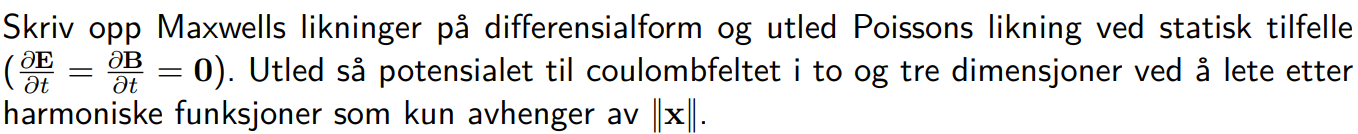
\includegraphics[width=0.7 \textwidth]{./02.png}
    \caption{}
    \label{fig:02}
\end{figure}
Maxwells likninger på differensialform er:

\begin{enumerate}
\item Gauss' lov for elektrisitet: $\nabla \cdot \mathbf{E} = \frac{\rho}{\epsilon_0}$.
\item Gauss' lov for magnetisme: $\nabla \cdot \mathbf{B} = 0$.
\item Faradays lov: $\nabla \times \mathbf{E} = -\frac{\partial \mathbf{B}}{\partial t}$.
\item Ampères lov med Maxwells tillegg: $c^2 \nabla \times \mathbf{B} = \frac{\partial \mathbf{E}}{\partial t} + \frac{\mathbf{J}}{\epsilon_0}$.
\end{enumerate}

Her er $\mathbf{E}$ det elektriske feltet, $\rho$ er ladningstettheten, $\epsilon_0$ er permittiviteten til vakuum, $\mathbf{B}$ er det magnetiske feltet, $t$ er tid, $c$ er lysets hastighet, og $\mathbf{J}$ er strømtettheten.

For det statiske tilfellet, der $\frac{\partial \mathbf{E}}{\partial t}=\frac{\partial \mathbf{B}}{\partial t}=\mathbf{0}$, blir Ampères lov med Maxwells tillegg redusert til

\begin{equation*}
c^2 \nabla \times \mathbf{B} = \frac{\mathbf{J}}{\epsilon_0}
\end{equation*}

og Faradays lov blir redusert til

\begin{equation*}
\nabla \times \mathbf{E} = \mathbf{0}
\end{equation*}

som indikerer at det elektriske feltet er konservativt, og det kan uttrykkes som gradienten av et potensial $\phi$, så $\mathbf{E} = -\nabla \phi$. Ved å sette dette i Gauss' lov får vi Poissons likning:

\begin{equation*}
\nabla^2 \phi = - \frac{\rho}{\epsilon_0}
\end{equation*}

Dette er Poissons likning for det elektriske potensialet $\phi$ i et område med ladningstetthet $\rho$.


Vi kan løse Poissons likning ved å bruke metoden for separasjon av variabler. Løsningen vi søker er av formen $\phi(r)$, der $r$ er avstanden fra origo.

Poissons likning i sfærisk koordinatsystem er:

\begin{equation*}
\nabla^2 \phi = \frac{1}{r^2} \frac{\partial}{\partial r} \left(r^2 \frac{\partial \phi}{\partial r}\right) = - \frac{\rho}{\epsilon_0}
\end{equation*}

Her tar vi utgangspunkt i en punktladning, der ladningstettheten $\rho = q \delta(\mathbf{r})$. Her er $q$ ladningen og $\delta$ er Diracs delta-funksjon.

Vi setter dette inn i Poissons likning:

\begin{equation*}
\frac{1}{r^2} \frac{\partial}{\partial r} \left(r^2 \frac{\partial \phi}{\partial r}\right) = - \frac{q}{\epsilon_0} \delta(\mathbf{r})
\end{equation*}

Løsningen av denne likningen i tre dimensjoner er kjent som Coulombs lov, og gir potensialet for en punktladning som:

\begin{equation*}
\phi(r) = \frac{1}{4\pi\epsilon_0} \frac{q}{r}
\end{equation*}

For to dimensjoner, er den radiale delen av Laplace-operator noe forskjellig, og Poissons likning blir:

\begin{equation*}
\nabla^2 \phi = \frac{1}{r} \frac{\partial}{\partial r} \left(r \frac{\partial \phi}{\partial r}\right) = - \frac{\rho}{\epsilon_0}
\end{equation*}

Setter vi inn for $\rho = q \delta(\mathbf{r})$ får vi:

\begin{equation*}
\frac{1}{r} \frac{\partial}{\partial r} \left(r \frac{\partial \phi}{\partial r}\right) = - \frac{q}{\epsilon_0} \delta(\mathbf{r})
\end{equation*}

Løsningen av denne likningen i to dimensjoner gir potensialet for en punktladning som:

\begin{equation*}
\phi(r) = \frac{1}{2\pi\epsilon_0} q \ln(r)
\end{equation*}

Husk at disse løsningene er avledet under antagelsen om isotropi, dvs. at feltet ikke har noen foretrukken retning. I et virkelig fysisk system må man ta hensyn til eventuelle grensebetingelser.



Formulering av Poissons likning i sfærisk koordinatsystem: Dette er et viktig første skritt fordi vi forventer at potensialet vil avhenge bare av avstanden fra origo, noe som er naturlig å uttrykke i sfæriske koordinater. Poissons likning i sfærisk koordinatsystem er:

\begin{equation*}
\nabla^2 \phi = \frac{1}{r^2} \frac{\partial}{\partial r} \left(r^2 \frac{\partial \phi}{\partial r}\right) = - \frac{\rho}{\epsilon_0}
\end{equation*}

Antagelse om punktladning: Vi forenkler problemet ved å anta at det elektriske feltet er produsert av en punktladning. Dette betyr at ladningstettheten $\rho$ er lik $q \delta(\mathbf{r})$, hvor $q$ er ladningen og $\delta$ er Diracs delta-funksjon som beskriver en punktladning.

Dirac delta-funksjonen, $\delta(\mathbf{r})$, er en matematisk funksjon som er null overalt bortsett fra i origo, og har den egenskapen at dens integral over hele rommet er lik 1. Dette gjør den veldig nyttig for å beskrive fysiske situasjoner der en gitt størrelse er konsentrert i et enkelt punkt i rommet, som i vårt tilfelle, hvor vi har en punktladning.

Sette inn punktladningen i Poissons likning: Nå setter vi inn uttrykket for $\rho$ i Poissons likning. Poissons likning er:

\begin{equation*}
\nabla^2 \phi = -\frac{\rho}{\epsilon_0}
\end{equation*}

Vi setter inn uttrykket for $\rho$ fra punkt 2 og får:

\begin{equation*}
\nabla^2 \phi = -\frac{q \delta(\mathbf{r})}{\epsilon_0}
\end{equation*}

eller ved å omforme litt:

\begin{equation*}
\frac{1}{r^2} \frac{\partial}{\partial r} \left(r^2 \frac{\partial \phi}{\partial r}\right) = - \frac{q}{\epsilon_0} \delta(\mathbf{r})
\end{equation*}

Denne likningen uttrykker nå hvordan det elektriske potensialet $\phi$ varierer i rommet rundt en punktladning.

Løsning av differensiallikningen: Dette er en differensiallikning som kan løses ved å integrere begge sider. Merk at høyresiden av likningen blir null for alle $r \neq 0$ på grunn av Dirac delta-funksjonen. Dette gir oss to separate likninger å løse, én for $r > 0$ og én for $r < 0$. Disse to løsningene må deretter matches ved $r = 0$ på en måte som er konsistent med tilstedeværelsen av delta-funksjonen.

For $r \neq 0$ har vi likningen:

\begin{equation*}
\frac{1}{r^2} \frac{\partial}{\partial r} \left(r^2 \frac{\partial \phi}{\partial r}\right) = 0
\end{equation*}

som har løsningen $\phi(r) = A \ln(r) + B$ der A og B er konstanter.

For å bestemme konstantene, merker vi oss at for $r \neq 0$ må det elektriske feltet være endelig og at det skal være kontinuerlig i $r = 0$. Dette betyr at løsningen ikke kan inneholde $\ln(r)$-termen, så $A = 0$.

Vi sitter da igjen med $\phi(r) = B$, hvor B er en konstant som skal bestemmes. Merk at dette er løsningen for både $r > 0$ og $r < 0$ siden de begge må matche ved $r = 0$.

For å bestemme konstanten B, integrerer vi Poissons likning over et sfærisk volum med radius $\epsilon$, og lar deretter $\epsilon \rightarrow 0$. Dette gir oss verdien av B som $B = \frac{q}{4\pi\epsilon_0 r}$.

Dermed er løsningen av Poissons likning i tre dimensjoner:

\begin{equation*}
\phi(r) = \frac{q}{4\pi\epsilon_0 r}
\end{equation*}

Dette uttrykket gir det elektriske potensialet som en funksjon av avstanden $r$ fra ladningen.

Tilpassing for to dimensjoner: I to dimensjoner er den radiale delen av Laplace-operatoren litt forskjellig, og Poissons likning blir:

\begin{equation*}
\nabla^2 \phi = \frac{1}{r} \frac{\partial}{\partial r} \left(r \frac{\partial \phi}{\partial r}\right) = - \frac{\rho}{\epsilon_0}
\end{equation*}

Vi setter igjen inn for $\rho = q \delta(\mathbf{r})$:

\begin{equation*}
\frac{1}{r} \frac{\partial}{\partial r} \left(r \frac{\partial \phi}{\partial r}\right) = - \frac{q}{\epsilon_0} \delta(\mathbf{r})
\end{equation*}

Tilpassing for to dimensjoner: I to dimensjoner er den radiale delen av Laplace-operatoren litt forskjellig, og Poissons likning blir:

\begin{equation*}
\nabla^2 \phi = \frac{1}{r} \frac{\partial}{\partial r} \left(r \frac{\partial \phi}{\partial r}\right) = - \frac{\rho}{\epsilon_0}
\end{equation*}

For å forstå denne endringen, må vi tenke på hvordan den deriverte virker i to dimensjoner sammenlignet med tre dimensjoner. Laplace-operatoren, $\nabla^2$, beskriver en andreordens derivasjon i rommet. I tre dimensjoner, som vi har sett tidligere, er dette gitt ved den første ligningen i punkt 1. I to dimensjoner, derimot, mister vi en av de romlige dimensjonene, og Laplace-operatoren blir derfor forskjellig. Dette gjenspeiles i det nye uttrykket for Poissons likning.

Vi setter igjen inn for $\rho = q \delta(\mathbf{r})$:

\begin{equation*}
\frac{1}{r} \frac{\partial}{\partial r} \left(r \frac{\partial \phi}{\partial r}\right) = - \frac{q}{\epsilon_0} \delta(\mathbf{r})
\end{equation*}

Denne ligningen kan løses på en lignende måte som i tre dimensjoner. Vi observerer igjen at høyresiden av ligningen er null for alle $r \neq 0$.

Dette gir oss likningen for $r \neq 0$:

\begin{equation*}
\frac{1}{r} \frac{\partial}{\partial r} \left(r \frac{\partial \phi}{\partial r}\right) = 0
\end{equation*}

Vi har nå løst Poissons likning for $r \neq 0$ i to dimensjoner og funnet at den mest generelle løsningen er på formen

\begin{equation}
\phi(r) = A \ln(r) + B
\end{equation}

der A og B er konstanter som skal bestemmes. La oss undersøke disse konstantene mer detaljert.

Bestemmelse av B

For det første er det viktig å merke seg at det elektriske potensialet skal være endelig for alle verdier av $r$. Hvis vi ser på den logaritmiske termen i løsningen vår, ser vi at den går mot uendelig når $r$ går mot 0. Dette vil føre til en uendelig verdi for det elektriske potensialet ved $r = 0$, noe som fysisk ikke er akseptabelt. Derfor må vi kreve at konstanten A er null for å unngå denne uendeligheten. Dette gir oss B = 0.

Bestemmelse av A

For å bestemme konstanten A, kan vi integrere begge sider av Poissons likning over et sirkulært område med radius $\epsilon$, og deretter la $\epsilon$ gå mot 0. Vi får da:

\begin{equation}
\int \frac{1}{r} \frac{\partial}{\partial r} \left(r \frac{\partial \phi}{\partial r}\right) d^2r = - \frac{q}{\epsilon_0}
\end{equation}

Integrasjonen på venstre side blir lik $2\pi \epsilon A$, mens den på høyre side blir lik $-q/\epsilon_0$ når vi lar $\epsilon$ gå mot 0. Ved å sette disse to uttrykkene lik hverandre, får vi:

\begin{equation}
2\pi \epsilon A = - \frac{q}{\epsilon_0}
\end{equation}

Som løser til:

\begin{equation}
A = \frac{q}{2\pi\epsilon_0}
\end{equation}

Så den endelige løsningen av Poissons likning i to dimensjoner blir:

\begin{equation}
\phi(r) = \frac{q}{2\pi\epsilon_0} \ln(r)
\end{equation}

Dette gir det elektriske potensialet fra en punktladning i to dimensjoner.

Denne løsningen representerer potensialet fra en punktladning i to dimensjoner. Forskjellen mellom to og tre dimensjoner skyldes hvordan feltlinjene sprer seg i rommet. I tre dimensjoner sprer feltlinjene seg ut over overflaten av en sfære, mens i to dimensjoner sprer de seg over omkretsen av en sirkel.